% This template was initially provided by Dulip Withanage.
% Modifications for the database systems research group
% were made by Conny Junghans,  Jannik Strtgen and Michael Gertz

\documentclass[
     12pt,         % font size
     a4paper,      % paper format
     BCOR=10mm,version=first,     % binding correction
     DIV=14,version=first,        % stripe size for margin calculation
%     liststotoc,   % table listing in toc
%     bibtotoc,     % bibliography in toc
%     idxtotoc,     % index in toc
%     parskip       % paragraph skip instead of paragraph indent
     ]{scrreprt}

%%%%%%%%%%%%%%%%%%%%%%%%%%%%%%%%%%%%%%%%%%%%%%%%%%%%%%%%%%%%

% PACKAGES:

% Use German :
\usepackage[english]{babel}
% Input and font encoding
\usepackage[utf8]{inputenc}
\usepackage[T1]{fontenc}
% Index-generation
\usepackage{makeidx}
% Einbinden von URLs:
\usepackage{url}
% Special \LaTex symbols (e.g. \BibTeX):
%\usepackage{doc}
% Include Graphic-files:
\usepackage{graphicx}
% Include doc++ generated tex-files:
%\usepackage{docxx}
% Include PDF links
%\usepackage[pdftex, bookmarks=true]{hyperref}
\usepackage{csquotes}
\usepackage{color, colortbl, tabularx, ragged2e}
\definecolor{LightCyan}{rgb}{0.88,1,1}
\newcolumntype{C}{>{\raggedright\arraybackslash}X} % centered "X" column
% Fuer anderthalbzeiligen Textsatz
\usepackage{setspace}
\usepackage{multirow}
\usepackage{longtable}
\usepackage{float}
\usepackage{wrapfig}
\usepackage{subfiles} % Best loaded last in the preamble

% hyperrefs in the documents
\usepackage[bookmarks=true,colorlinks,pdfpagelabels,pdfstartview = FitH,bookmarksopen = true,bookmarksnumbered = true,linkcolor = black,plainpages = false,hypertexnames = false,citecolor = black,urlcolor=black]{hyperref} 
%\usepackage{hyperref}


%%%%%%%%%%%%%%%%%%%%%%%%%%%%%%%%%%%%%%%%%%%%%%%%%%%%%%%%%%%%

% OTHER SETTINGS:

% Pagestyle:
\pagestyle{headings}

% Choose language
\newcommand{\setlang}[1]{\selectlanguage{#1}\nonfrenchspacing}

\usepackage{biblatex}
\addbibresource{references.bib}

\begin{document}

% TITLE:
\pagenumbering{roman}
\begin{titlepage}
     \vspace*{1cm}
     \begin{center}
          \vspace*{3cm}
          \textbf
          {
               \Large University of Heidelberg\\
               \smallskip
               \Large Institute for Computer Science\\
               \smallskip
               \Large Working group database systems\\
               \smallskip
          }

          \vspace{3cm}

          \textbf{\large Bachelor thesis}

          \vspace{0.5\baselineskip}
          {
               \huge
               \textbf{Integrating Identity Management Providers based on Online Zugangs Gesetz}
          }

     \end{center}

     \vfill
     {
          \large
          \begin{tabular}[l]{ll}
               Name:                 & Jonas Gann              \\
               Matriculation number: & 3367576                 \\
               Supervisor:           & Prof. Dr. Michael Gertz \\
               Date of submission:   & \today
          \end{tabular}
     }

\end{titlepage}

\onehalfspacing

\thispagestyle{empty}

\vspace*{100pt}
\noindent
I assure that I have written this bachelor thesis on my own and only used the specified sources and resources and that I followed the principles and recommendations "Responsibility in Science" of the University of Heidelberg.

\vspace*{50pt}
\noindent

\underline{\phantom{mmmmmmmmmmmmmmmmmmmm}}

\medskip
\noindent
Date of Submission: \today
\newpage

\chapter*{Zusammenfassung}

\newpage

\chapter*{Abstract}

\newpage

\tableofcontents
\cleardoublepage
\pagenumbering{arabic}

\chapter{Introduction}

\section{Context}

\subfile{sections/1-context}

\section{Objective}

\subfile{sections/2-objective}

\section{Structure of Work}

\subfile{sections/3-structure_of_work}

\chapter{Background and Related Work}

\section{Terminology}

\subfile{sections/4-terminology}

\section{Online Access Law (OZG)}

\subfile{sections/5-online_access_law}

\section{Messaging}

This section describes possibilities of constructing a message based integration architecture

\subsection{Messaging Patterns}

\chapter{Identity Management}

\section{Functional Requirement Analysis}


\subfile{sections/6-requirement_analysis}

\section{IMP System Solution}

\subfile{sections/7-imp_system_proposal}

\chapter{Integration Challenges}

This chapter describes challenges for integrating the IMP system described in chapter 3 into the OZG system architecture. The quality of the presented integration can be determined based on the number of the following challenges it solves.

\section{IMP Challenges}
This section describes challenges which arise from the operation of the IMP system

\begin{itemize}
    \item Connector has REST interface and cannot notify system architecture
    \item Connector does not understand messages
    \item Messages can have different versions
    \item API of connector can change
    \item New types of messages can be added by the client and the system provider might need to understand them
\end{itemize}

\section{SP Challenges}

This section describes challenges which arise from service provider integration requirements.

\begin{itemize}
    \item Minimal modification of existing systems
    \item Maintainability
    \item Scalability
    \item Failure Handling
    \item Administration
    \item Extendability
    \item Modularity
    
\end{itemize}

\subsection{OZG Challenges}

This section describes challenges which arise from OZG integration requirements.

\begin{itemize}
    \item Administration portal has access to all personal information
    \item Once an application is submitted, its attributes cannot be changed
    \item Mapping of IMP attributes and FIM data blocks
    \item Messages can have a correlation (request-reply) which the system architecture might want to keep track of
\end{itemize}

\chapter{Initial Solution Proposal}

The goal of the initial integration solution is to introduce features of the IMP system into the OZG system architecture. All existing services should be accessible the same way as before but with additional options for using IMP. The focus of this initial integration is to avoid disruption of existing system operation through non-invasive integration, to enable a fast and simple entrance into the IMP system and to provide future upgrade capabilities. The integration takes place on three layers:

\begin{figure}[h]
\caption{IMP Layer Diagram}
    \centering
    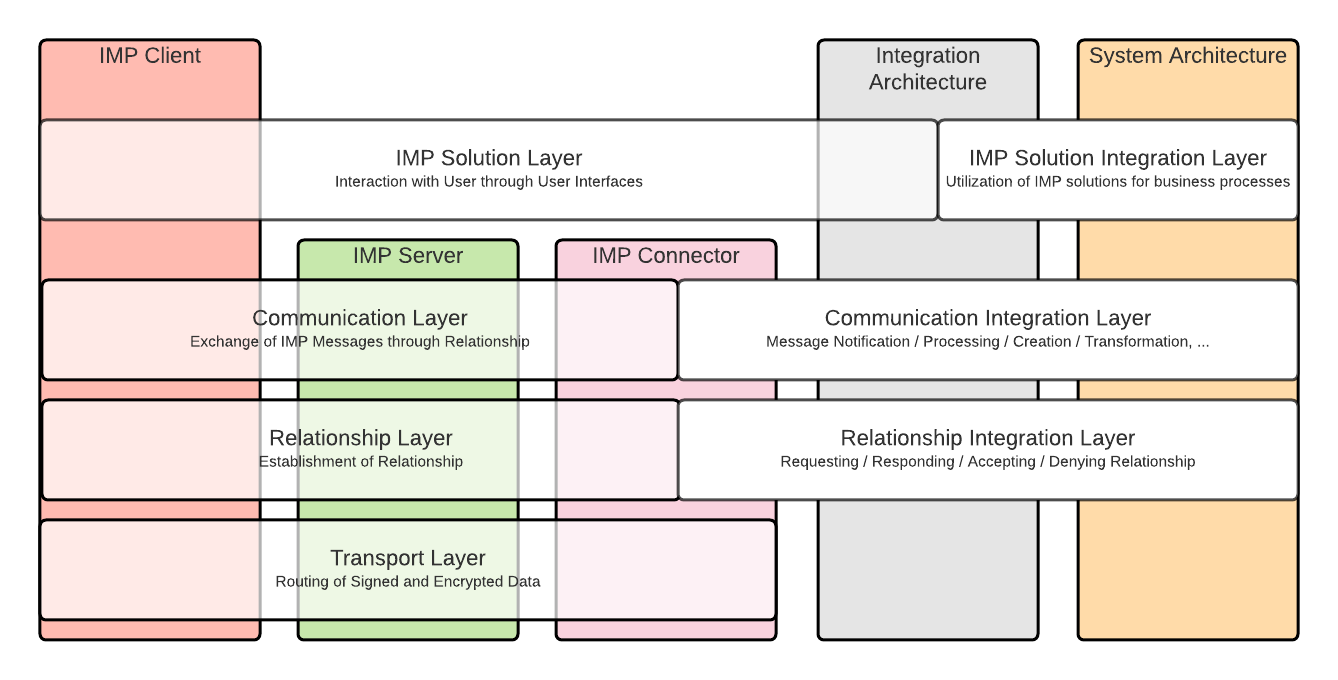
\includegraphics[scale=0.3]{Diagrams/Integration Architecture 1/IMP Layer Diagram Integration.png}
\end{figure}

\paragraph{IMP Solution Integration Layer} 
The purpose of the integration on the IMP solution layer is to take advantage of new interaction capabilities with the user through the IMP system. Chapter 3 gives some examples on how the IMP client can enable the user to interact with the IMP system. The integration evaluates possibilities of using relationships and IMP messages to improve OZG services, defines what the purpose of each message and relationship type is and how they should be handled by client and service provider. For example relationship templates can be defined and new message types can be created with corresponding new user interfaces in the IMP client.

\paragraph{Relationship Integration Layer} The purpose of the integration on the relationship layer is to enable the technological utilization of relationships as described by the integration on the solution integration layer. 

\paragraph{Communication Integration Layer} The purpose of the integration on the communication layer is to enable the technological utilization of messages as described by the integration on the solution integration layer. 

\section{IMP Solution Integration}

\subfile{sections/8-imp_solution_integration}

\section{Technological Integration}

This section evaluates possibilities of a technological integration architecture for realizing the integration solution described in the previous section.

\subfile{sections/9-technological_integration}


\chapter{Advanced Solution Proposal}

The goal of this integration architecture is to make as much functionalities required for the basic OZG use case available through the IMP client. Now, the OZG user profiles are replaced with IMP identities and the integration architecture integrates with any system component necessary.

\begin{figure}[h]
    \centering
    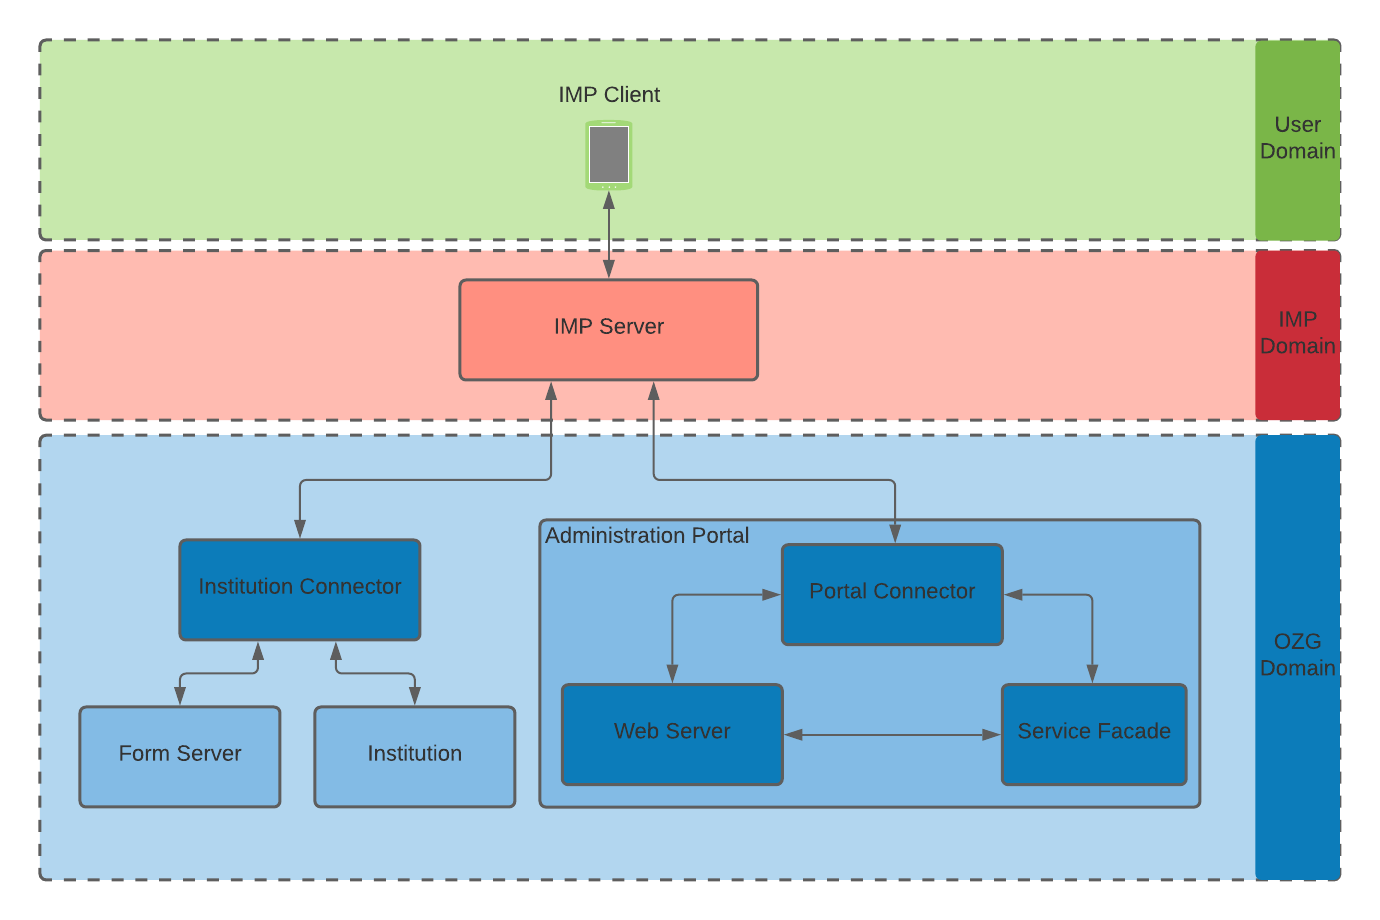
\includegraphics[scale=0.15]{Diagrams/Integration Architecture 2/Overview.png}
\end{figure}

\section{IMP Solution Integration}

\subfile{sections/10-imp_solution_integration}

\chapter{Solution Evaluation}

\section{Conclusion}

\chapter{Outlook: Advanced IMP Integration}


\printbibliography


\end{document}
